%!TEX root = ../main.tex

\chapter{Schematic Editor}

The first step in every project is schematic capture.
If this term is unfamiliar, we are referring to the process of laying out the components and connections between them in logical, well-defined fashion.
You may have only the barest idea of the circuit aspects or you may have the major aspects already sketched on paper;
whatever your situation, transferring the schematic into KiCad begins with the Schematic Editor.

Before we dive into the simplistic aspects of the schematic editor, it will pay us dividends later to properly understand how the schematic editor views more complex schematics.
This will allow you to structure the schematic in your mind more closely to how Schematic Editor expects.

\section{Hierarchical Schematics Explained}

The basic, underlying paradigm of the Schematic Editor is the idea of \textit{hierarchical schematics}.
If the overall schematic represents the full circuit that will exist on the circuit board at the end of production, then the hierarchy provides a logical grouping of similar component sets.
This allows you to reuse common subsets throughout your design.
The hierarchy also explicitly structures your schematics as a top-down tree.
\begin{figure}
	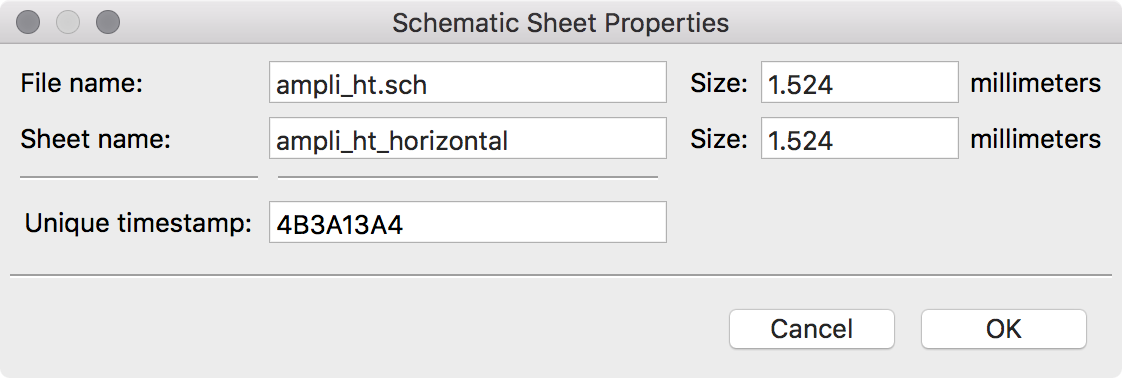
\includegraphics{chapter5/subsheet.png}
	\caption[Sub-Sheets]{The subsheet dialog specifies the file name, sheet name and a unique timestamp.}
\end{figure}

At the root of the tree, is the first schematic sheet you open, usually with the same name as your project and the extension `\textbf{.sch}'.
Off of this root, you can create \textit{sub-sheets} that are placed in the root sheet.
The sub-sheet has both a ``File name'' and a ``Sheet name''.
The File name is the name of the sub-sheet on the underlying filesystem.
This is the name you will see if you open your project folder outside of KiCad.
The Sheet name is the internal reference of the specific \textit{instance} of the sub-sheet in KiCad.

One of the primary benefits of this setup is the ability to organize the relationship between subsheets.
Instead of utilizing global net labels to connect disparate elements between sheets, you can use hierarchical subsheets layout the explicit connection between schematic elements.

It can also allow you to create and re-use common elements through and between projects.
This will be useful when we begin discussing design reuse in section \ref{sec:reuse}.



\section{Understanding the Schematic Editor}

When you first open the schematic editor, you are presented with a blizzard of information.
In KiCad, the majority of functions are accessed using buttons and hotkeys.
Unlike many programs, where functionality is often buried in sub-menus, KiCad prefers to expose its controls up front.
This has the benefit of providing easy access to virtually all commands, and the drawback of an overwhelming first impression.

\begin{figure*}
    \begin{tikzpicture}[baseline]
    \begin{scope}
        \node[anchor=south west,inner sep=0] (image) at (0,0) 
        	{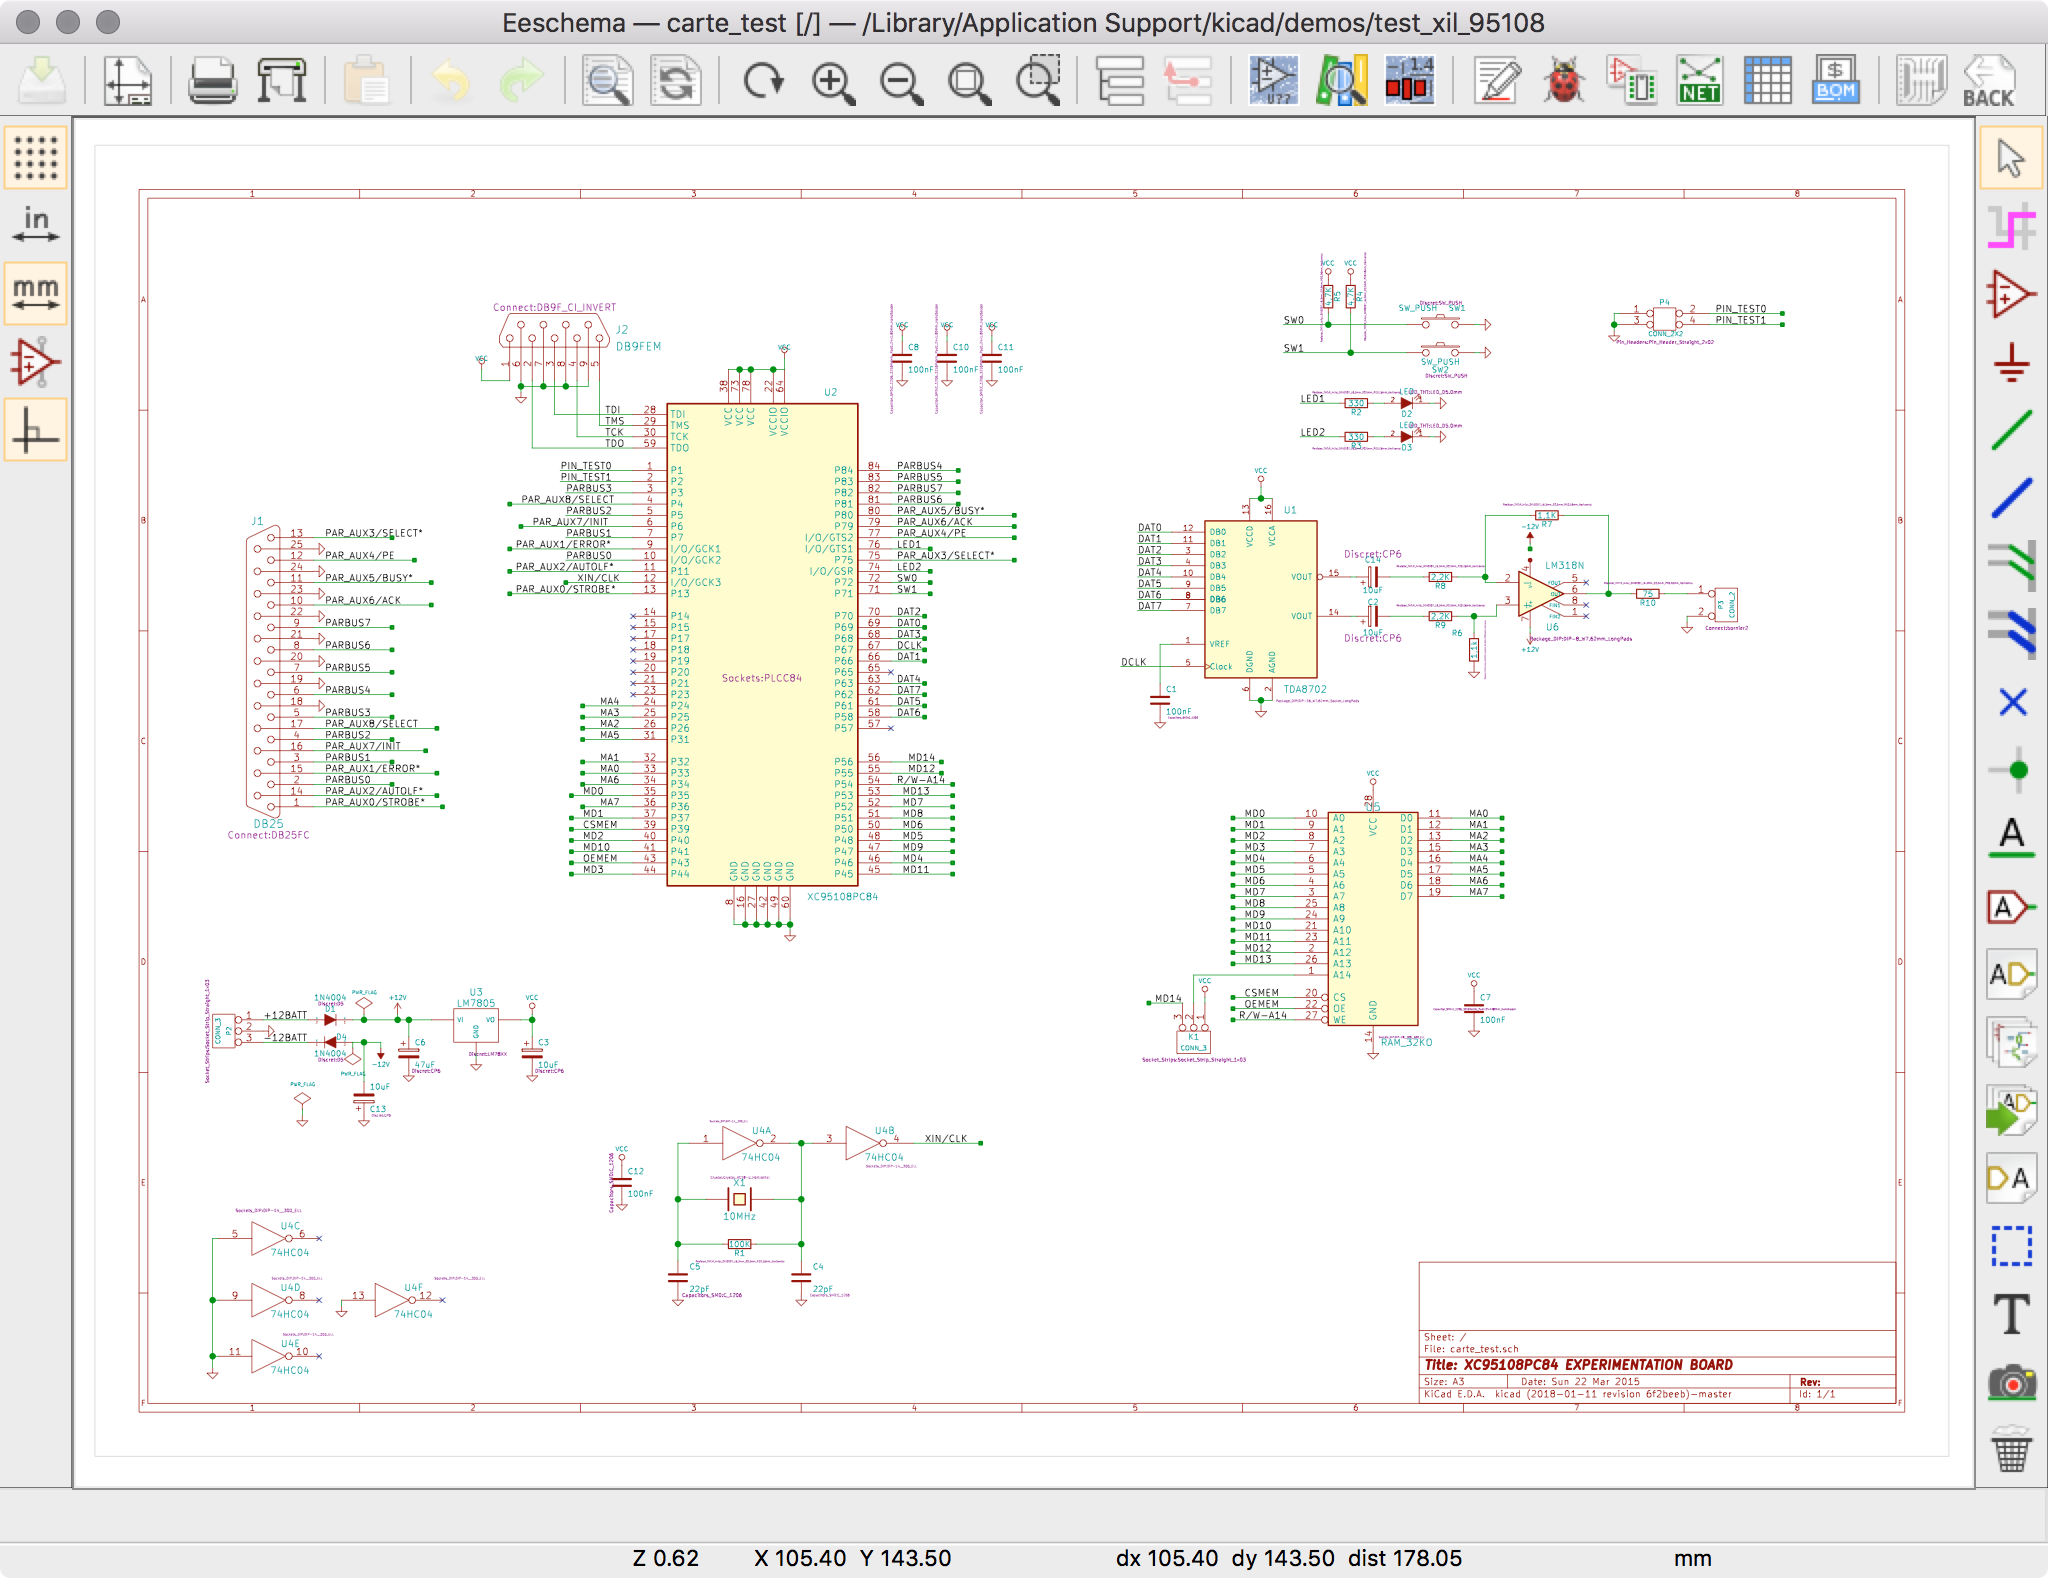
\includegraphics[width=4.5in]{chapter5/eeschema-main.png}};
        \begin{scope}[x={(image.south east)},y={(image.north west)}]
            \node [anchor=south] (file) at (0.08,1.0) {\large File\strut };
            \node [anchor=south] (edit) at (0.2575,1.0) {\large Edit\strut };
            \node [anchor=south] (view) at (0.438,1.0) {\large View\strut };
            \node [anchor=south] (app) at (0.763,1.0) {\large Applications\strut };
            \node [anchor=south, rotate=-90] (tools) at (1.0,0.5) {\large Schematic Tools};
            \node [anchor=north, rotate=-90] (options) at (0.0,0.5) {\large Display Options};
            \node [above left=-2pt] (coord) at (0.0,0.0) {\large Coordinates };
            
%            \draw[help lines,xstep=.05,ystep=.05] (0,0) grid (1,1);
            \draw[red,thick,rounded corners] (0.0,0.923) rectangle (0.155,0.97);
            \draw[red,thick,rounded corners] (0.162,0.923) rectangle (0.35,0.97);
            \draw[red,thick,rounded corners] (0.357,0.923) rectangle (0.525,0.97);
            \draw[red,thick,rounded corners] (0.60,0.923) rectangle (1.0,0.97);
            \draw[black!80,thick, dashed, rounded corners] (0.961,0.92) rectangle (1.0,0.05);
            \draw[black!80,thick, dashed, rounded corners] (0.0,0.92) rectangle (0.039,0.7);
            \draw [-latex, thick, red] ([yshift=-2pt]file.base) -- ++(0,-0.05);
            \draw [-latex, thick, red] ([yshift=-2pt]view.base) -- ++(0,-0.05);
            \draw [-latex, thick, red] ([yshift=-2pt]edit.base) -- ++(0,-0.05);
            \draw [-latex, thick, red] ([yshift=-2pt]app.base) -- ++(0,-0.05);
            \draw [-latex, thick, dashed, black!80] (tools.west) to[out=90, in=-20] (1.0,0.85);
            \draw [-latex, thick, dashed, black!80] (options.west) to[out=90, in=-160] (0.0,0.85);
            \draw [-latex, thick, dotted, black!80] (coord.east) -- ++(0.15,0.0);
        \end{scope}
    \end{scope}
    \end{tikzpicture}
	
	\caption[fig:eeschema]{The Eeschema main window.  Control and execution buttons are on the top, options buttons are in the left vertical bar and tools buttons are in the right vertical bar. }
\end{figure*}

Looking at the Eeschema window in Figure \ref{fig:eeschema}, you can see this division.
The ``Display Options'' toolbar on the left consists of buttons and are either enabled or disabled, depending on your working preferences.

\newpage
\begin{marginfigure}
	\tcbset{nobeforeafter}
	\hfill\iconbox{\includesvg[width=7.5mm]{grid.svg}}
	\hfill\;
	\caption{Enable/Disable Grid Button}
\end{marginfigure}
The first icon is a grid and controls whether the grid dots are shown on the schematic or not.
Note that this does not change whether your elements snap to the grid; this is always enabled for Eeschema.

\begin{marginfigure}
	\tcbset{nobeforeafter}
	\hfill\iconbox{\includesvg[width=7.5mm]{unit_inch.svg}}
	\hfill\iconbox{\includesvg[width=7.5mm]{unit_mm.svg}}
	\hfill\;
	\caption{Units Selection Buttons}
\end{marginfigure}
The next two icons select either imperial (inch and mil) or metric (millimeter) units for the dimensions.  
When selecting one of these icons, you don't change the grid size, just the representation.
Note that while you can change the representation of the grid size, you cannot change the base unit.
That is to say, the grid is always in units of mil (thousandth of an inch) and their multiples.
This is an historical artifact of the underlying schematic format.
\sidenote{Originally, Eeschema and Pcbnew used similar file formats.  
When they were designed in the early 1990s, the vast majority of components were only available in imperial pitch.
Therefore it made sense to have the base unit be the mil.
This limitation no longer exists for pcbnew and there are plans in the works to change it for Eeschema in version 6.}

\begin{marginfigure}
	\tcbset{nobeforeafter}
	\hfill\iconbox{\includesvg[width=7.5mm]{cursor_shape.svg}}
	\hfill\;
	\caption{Cursor Shape Buttons}
\end{marginfigure}
The next icon selects the cursor shape for Eeschema.
Enabling this button will change the cursor shape to a cross-hair whose whiskers extend across the canvas.
\sidenote{This option is not available on the MacOS version.}


\begin{marginfigure}
	\tcbset{nobeforeafter}
	\hfill\iconbox{\includesvg[width=7.5mm]{hidden_pin.svg}}
	\hfill\;
	\caption{Show Hidden Pins Buttons}
\end{marginfigure}
Eeschema allows pins to be hidden on components.
Hidden pins are useful for multiple pins that share functions and pins that are not meant to be connected\cite{http://kicad-pcb.org/libraries/klc/S4.6/}.
Historically, hidden pins were also used for common connection pins such as \textbf{VCC} or \textbf{GND}.
This caused many issues as Eeschema connects hidden pins to wires that cross them, so users would sometimes find their netlist cross-linked by a wire that inadvertently crossed a hidden pin.
While new library symbols in the official distribution have explicitly separated the hidden connection pins per KLC4.6, there exist some historical symbols, notably in the \textit{Logic\_TTL\_IEEE} and \textit{Logic\_74xgxx} libraries that have not be updated to the new standard.
Selecting this view option is a good way to verify you haven't been caught by this particular issue

\subsection{Relationship to Symbol Libraries}
\subsection{Project Settings}

\section{Adding Parts}

\section{Connections}
\subsection{Wires}
\subsection{Busses}
\subsection{Labels}
\subsection{Junctions}
\subsection{No Connects}
\subsection{Hierarchical Pins}

\section{Electrical Rules Check}

\section{Graphical Elements}

\section{Templates}

\section{Schematic Editor Examples}
\subsection{Example 1: Single Page Schematic}
\subsection{Example 2: Hierarchical Schematic}